\documentclass[12pt]{article}
\usepackage[margin=2.5cm]{geometry}
\usepackage{enumerate}
\usepackage{amsfonts}
\usepackage{amsmath}
\usepackage{fancyhdr}
\usepackage{amsmath}
\usepackage{amssymb}
\usepackage{amsthm}
\usepackage{mdframed}
\usepackage{graphicx}
\usepackage{subcaption}
\usepackage{adjustbox}
\usepackage{listings}
\usepackage{xcolor}
\usepackage{courier}
\usepackage[utf]{kotex}
\usepackage{hyperref}
\usepackage{soul}
\usepackage{cancel}


\definecolor{codegreen}{rgb}{0,0.6,0}
\definecolor{codegray}{rgb}{0.5,0.5,0.5}
\definecolor{codepurple}{rgb}{0.58,0,0.82}
\definecolor{backcolour}{rgb}{0.95,0.95,0.92}

\lstdefinestyle{mystyle}{
    backgroundcolor=\color{backcolour},
    commentstyle=\color{codegreen},
    keywordstyle=\color{magenta},
    numberstyle=\tiny\color{codegray},
    stringstyle=\color{codepurple},
    basicstyle=\ttfamily\footnotesize,
    breakatwhitespace=false,
    breaklines=true,
    captionpos=b,
    keepspaces=true,
    numbers=left,
    numbersep=5pt,
    showspaces=false,
    showstringspaces=false,
    showtabs=false,
    tabsize=1
}

\lstset{style=mystyle}

\pagestyle{fancy}
\renewcommand{\headrulewidth}{0.4pt}
\lhead{CSC 369}
\rhead{Reading Notes}

\begin{document}
\title{CSC 369 Reading Notes}

\section{Limited Direct Execution}

\begin{mdframed}
\underline{\textbf{Vocabulary}}

\bigskip

\begin{enumerate}[1.]
    \item \textbf{Time Sharing}
    \begin{itemize}
        \item Is a mechanism used by an OS to share a resource
        \item Allows an entity to use the resource for a little while, and then
        a little while by another, and so forth

        \bigskip

        \underline{\textbf{Example}}

        \bigskip

        CPU
    \end{itemize}
    \item \textbf{Limited Direct Execution}
    \begin{itemize}
        \item Is synomyous to \textbf{baby proofing}
        \item \textbf{Limited} Means there will be a limit to what a processor can and cannot do
        \item \textbf{Direct Execution} Means that the processor will run directly on the CPU
    \end{itemize}
    \item \textbf{User Mode}
    \begin{itemize}
        \item Is a processor mode where code that runs is restricted in what it can do
    \end{itemize}
    \item \textbf{Kernel Mode}
    \begin{itemize}
        \item Is a processor mode where code that runs can do what it likes, including
        previleged operations

        \bigskip

        \underline{\textbf{Example}}

        \bigskip

        Previleged operations include

        \begin{enumerate}[1.]
            \item I/O requests
            \item Executing all types of restricted instructions
        \end{enumerate}
    \end{itemize}
    \item \textbf{System Call}
    \begin{itemize}
        \item Is a programmatic way in which a computer program requests a previleged
        service from the kernel of the operating system
    \end{itemize}
    \item \textbf{Trap}
    \begin{itemize}
        \item Is a type of synchronous interrupt caused by an exceptional condition that
        \item Exceptional condition include:
        \begin{itemize}
            \item Breakpoint
            \item Division by zero
            \item Invalid memory access
            \item System Call
        \end{itemize}
        \item Usually results in a processor switching to kernel mode
    \end{itemize}
    \item \textbf{Return-from-Trap}
    \begin{itemize}
        \item Is an instruction that
        \begin{itemize}
            \item Restores saved registers from kernel stack
            \item Swithces the processor back to \textbf{user mode}
        \end{itemize}
    \end{itemize}
    \item \textbf{Trap Table}
    \begin{itemize}
        \item [\color{blue}Question\color{black}] What is the exact definition of a trap table? OSTEP
        glosses over it :(
        \item Is synonymous to 대응 메뉴얼
        \item Is a list of trap handlers where each is associated with a specific trap
    \end{itemize}
    \item \textbf{Trap Handlers}
    \begin{itemize}
        \item Is the code that will run when the trap is triggered.
    \end{itemize}
    \item \textbf{System-call Number}
    \begin{itemize}
        \item Is an ID assigned to each system call

        \bigskip

        \begin{center}
        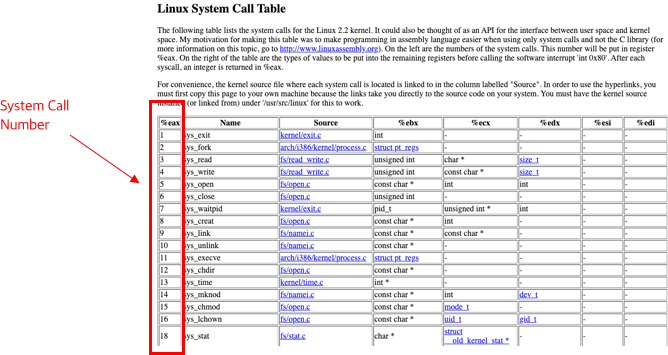
\includegraphics[width=0.9\linewidth]{images/notes_4_7.png}
        \end{center}
    \end{itemize}
    \item \textbf{Timer Interrupt}
    \begin{itemize}
        \item Is a type of interrupt generated by an internal clock instead of an external event (e.g I/O or system call)
    \end{itemize}
    \item \textbf{Interrupt Handler}
    \begin{itemize}
        \item Is a special block of code associated with a specific interrupt condition
    \end{itemize}
\end{enumerate}

\end{mdframed}

\subsection{Direct Execution}
\begin{itemize}
    \item Means just run program directly without limits
    \item Has advantage of being fast

    \begin{center}
    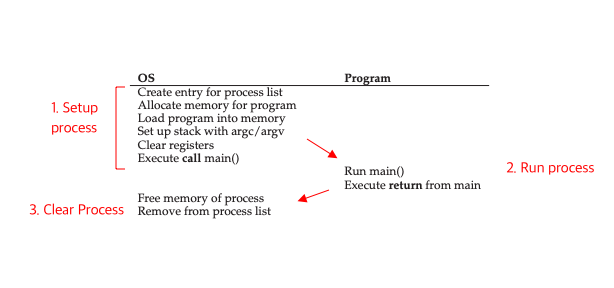
\includegraphics[width=0.6\linewidth]{images/notes_4_8.png}
    \end{center}
\end{itemize}

\subsection{Problem \#1: Restricted Operations}
\begin{itemize}
    \item \textbf{Question:} How can the OS make sure a program doesn't do anything that we
    don't want to do while running it efficiently?
    \item Solution
    \begin{itemize}
        \item \textbf{user mode}
        \item \textbf{kernel mode}
    \end{itemize}
    \item \textbf{Question \# 2:} What should a user process do when it wishes to perform
    some kind of previleged operation?
    \item Solution
    \begin{itemize}
        \item \textbf{system call}
    \end{itemize}

    \begin{center}
    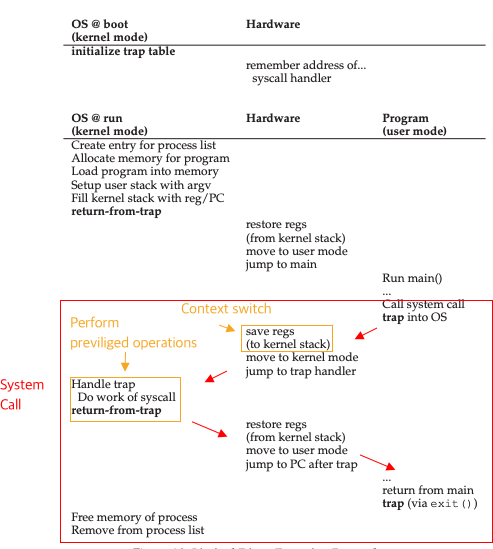
\includegraphics[width=0.6\linewidth]{images/notes_4_9.png}
    \end{center}
\end{itemize}

\subsection{Problem \#2: Switching Between Processes}
\begin{itemize}
    \item \textbf{Question:} When we are running a process, how does the oeprating system stop it
    from running and switch to another process, thus implementing \textbf{time sharing} mechanism
    to virtualize CPU?
\end{itemize}

\subsection{Concurrency}

\end{document}
